% Figure F1: the t-SNE method as a loop, with the step numbers used in Section 4 and Figure A1.
% Same colours and box style as method_map.tex. Build: tectonic -X compile method_loop.tex
\documentclass[border=1pt]{standalone}
\usepackage[T1]{fontenc}\usepackage{helvet}\renewcommand{\familydefault}{\sfdefault}
\usepackage{amsmath}
\usepackage{tikz}\usetikzlibrary{arrows.meta,positioning}
\definecolor{ink}{HTML}{1B2733}\definecolor{boxc}{HTML}{E4E9EF}\definecolor{datac}{HTML}{F4F6F8}
\begin{document}
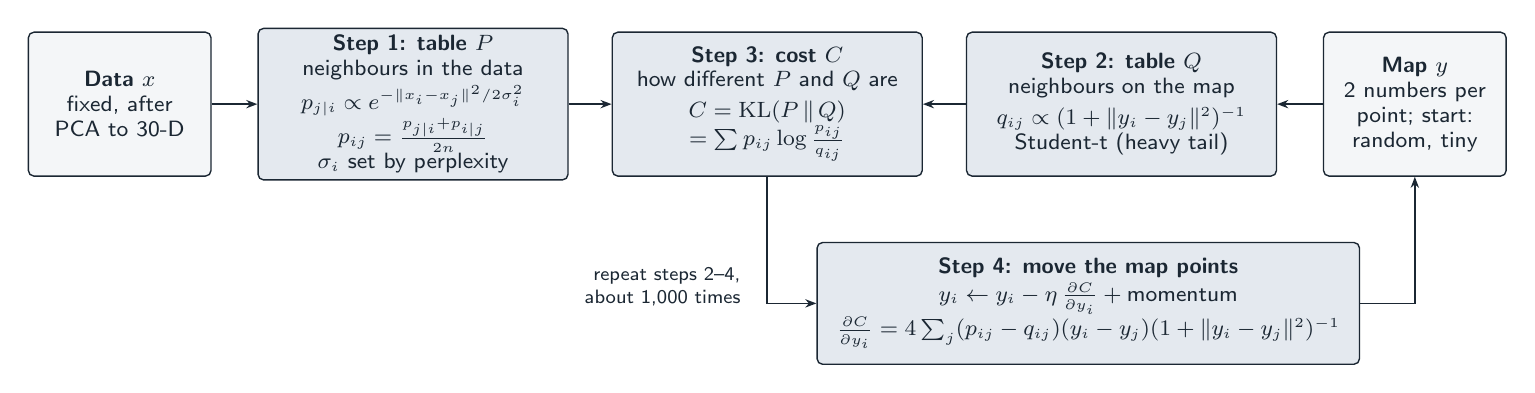
\begin{tikzpicture}[x=1pt,y=1pt,
 st/.style={draw=ink,line width=.5pt,rounded corners=2pt,fill=boxc,minimum width=112pt,minimum height=52pt,inner sep=2.5pt,align=center,text=ink,font=\fontsize{7.6}{9}\selectfont},
 dt/.style={st,fill=datac,minimum width=66pt},
 ar/.style={-{Stealth[length=4pt]},draw=ink,line width=.6pt},
 lab/.style={font=\fontsize{7}{8.2}\selectfont,text=ink,align=right,inner sep=1.5pt}]
% top row: data -> step 1 -> step 3 <- step 2 <- map points
\node[dt] (x) at (0,0) {\textbf{Data $x$}\\fixed, after\\PCA to 30-D};
\node[st] (p) at (106,0) {\textbf{Step 1: table $P$}\\neighbours in the data\\[1pt]
  $p_{j|i}\propto e^{-\|x_i-x_j\|^2/2\sigma_i^2}$\\
  $p_{ij}=\frac{p_{j|i}+p_{i|j}}{2n}$\\$\sigma_i$ set by perplexity};
\node[st] (c) at (234,0) {\textbf{Step 3: cost $C$}\\how different $P$ and $Q$ are\\[2pt]
  $C=\mathrm{KL}(P\,\|\,Q)$\\$=\sum p_{ij}\log\frac{p_{ij}}{q_{ij}}$};
\node[st] (q) at (362,0) {\textbf{Step 2: table $Q$}\\neighbours on the map\\[2pt]
  $q_{ij}\propto(1+\|y_i-y_j\|^2)^{-1}$\\Student-t (heavy tail)};
\node[dt] (y) at (468,0) {\textbf{Map $y$}\\2 numbers per\\point; start:\\random, tiny};
\draw[ar] (x)--(p); \draw[ar] (p)--(c); \draw[ar] (q)--(c); \draw[ar] (y)--(q);
% step 4 below, closing the loop
\node[st,minimum width=196pt,minimum height=44pt] (g) at (350,-72) {\textbf{Step 4: move the map points}\\[1pt]
  $y_i \leftarrow y_i-\eta\,\frac{\partial C}{\partial y_i}+\text{momentum}$\\
  $\frac{\partial C}{\partial y_i}=4\sum_j(p_{ij}-q_{ij})(y_i-y_j)(1+\|y_i-y_j\|^2)^{-1}$};
\draw[ar] (c.south) |- (g.west);
\draw[ar] (g.east) -| (y.south);
\node[lab,anchor=east] at (226,-66) {repeat steps 2--4,\\about 1{,}000 times};
\end{tikzpicture}
\end{document}
